% Provenance (never printed): see sources/outline_sources.md (Year 3:
% fractionation and Rayleigh distillation in the water cycle;
% palaeothermometry; carbon and sulfur isotopes). Brief:
% sources/book5/BRIEFS.md, ch. 14. Curves from figdata/bachelor-3/
% rayleigh_distillation.py, lr04_d18o.py, carbon_mass_balance.py. Exercise
% and problem values in the Book 5 scratch calculator calc/ch14.py. Dome Ilse,
% its traverse and the marine core are invented.
\chapter{Geoquímica de isótopos estables}\label{ch:b3:stable-isotopes}

La nieve que cae sobre las cúpulas altas del casquete de hielo de la Antártida Oriental está entre el
agua más ligera de la Tierra. Cada una de sus moléculas salió del océano como vapor, y
en el camino hacia el interior el aire perdió la mayor parte de su agua en forma de nieve, primero las moléculas pesadas.
Lo que queda a la llegada depende de cuánta se perdió, lo cual depende de
cuán fría llegó a estar la masa de aire. Una columna de hielo es, por tanto, un termómetro; una concha
de calcita otro, y el carbono de las calizas un registro de lo que la
biosfera enterró. Este capítulo deduce las leyes que hay detrás de estos registros y
los interpreta.

\begin{recall}
El valor $\delta$, el factor de fraccionamiento $\alpha$ y los efectos isotópicos de equilibrio y
cinéticos se estudian en los volúmenes universitarios de los libros de química. Los
estándares de referencia VSMOW y VPDB y la recta de agua meteórica se encuentran en el
volumen de segundo año, en su capítulo de geoquímica isotópica; la ley de
fraccionamiento de Rayleigh de los elementos traza en su capítulo sobre diferenciación magmática;
los indicadores climáticos, el efecto del volumen de hielo y el termómetro Mg/Ca
en su capítulo sobre archivos y indicadores climáticos; el
Máximo Térmico del Paleoceno-Eoceno en su capítulo sobre el clima a lo largo del
tiempo geológico; el Gran Evento de Oxidación en su capítulo sobre la Tierra precámbrica.
La fotosíntesis y la reducción bacteriana de sulfato se encuentran en los libros de biología.
\end{recall}

\section{Fraccionamiento entre dos fases}\label{sec:b3:stable-isotopes:fractionation}

Para dos fases A y B en equilibrio isotópico, $\alpha_{A-B} = R_A/R_B =
(1000 + \delta_A)/(1000 + \delta_B)$, con las razones $R$ del isótopo pesado al
ligero. El vapor de agua y el agua líquida tienen $\alpha = 1.0098$ para el oxígeno-18
y $1.084$ para el deuterio a \qty{20}{\celsius}, $1.0117$ y $1.111$ a
\qty{0}{\celsius}; el hielo y el agua a \qty{0}{\celsius}, $1.0035$ y $1.0208$.
La fase más pesada es siempre la más condensada, y el fraccionamiento
aumenta a medida que baja la temperatura.
% ledger: kc98:alpha, kc98:standards

\begin{definition}[Diferencia isotópica]\label{def:b3:stable-isotopes:big-delta}
La \emph{diferencia isotópica}\index{diferencia isotópica (delta mayúscula)}
entre dos fases es $\Delta_{A-B} = \delta_A - \delta_B$, en por mil.
\end{definition}

\begin{proposition}[Diferencia isotópica y factor de fraccionamiento]
\label{prop:b3:stable-isotopes:big-delta}
Para $\alpha$ próximo a 1 y valores pequeños de $\delta$,
\[
\Delta_{A-B} \approx 1000\ln\alpha_{A-B} \approx 1000(\alpha_{A-B} - 1).
\]
\end{proposition}

\begin{proof}
$1000\ln\alpha = 1000\ln(1 + \delta_A/1000) - 1000\ln(1 + \delta_B/1000)$, y
$1000\ln(1 + x/1000) = x - x^2/2000 + \dots$, por tanto $1000\ln\alpha = \delta_A -
\delta_B - (\delta_A^2 - \delta_B^2)/2000 + \dots$. Finalmente $\ln\alpha \approx
\alpha - 1$ para $\alpha$ cercano a 1.
\end{proof}

El error es $(\delta_A^2 - \delta_B^2)/2000$: una fracción de por mil con los
valores del océano, casi un por mil entre el océano y la nieve ligera del
hielo polar.
La magnitud $1000\ln\alpha$ es la que la teoría relaciona con la temperatura: varía
casi como $1/T^2$ a temperatura alta y como $1/T$ a baja,
y las calibraciones se escriben en esa forma. Para el hielo y el vapor, por ejemplo,
\[
\ln\alpha^{18}_{\mathrm{ice-v}} = \frac{11.839}{T} - 0.028224, \qquad
\ln\alpha^{\mathrm D}_{\mathrm{ice-v}} = \frac{16288}{T^2} - 0.0934,
\]
con $T$ en kelvins.
% ledger: gkinis14:alpha-ice, kc98:standards

\begin{definition}[Fraccionamiento dependiente e independiente de la masa]\label{def:b3:stable-isotopes:mif}
Un elemento con tres isótopos o más presenta un \emph{fraccionamiento dependiente
de la masa}\index{fraccionamiento dependiente de la masa} cuando los fraccionamientos de
sus razones isotópicas guardan la proporción de sus diferencias de masa, fijadas por las
masas; en caso contrario tiene un \emph{fraccionamiento independiente
de la masa}\index{fraccionamiento independiente de la masa}, medido por la desviación
respecto a la recta dependiente de la masa, como $\Delta^{33}\mathrm S = \delta^{33}\mathrm S
- 0.515\,\delta^{34}\mathrm S$.
\end{definition}

Para el oxígeno, el fraccionamiento de $^{17}\mathrm O/^{16}\mathrm O$ es aproximadamente 0.52 veces el de
$^{18}\mathrm O/^{16}\mathrm O$, próximo al cociente de las diferencias de masa, 1 a 2;
para el azufre, $\delta^{33}\mathrm S = 0.515\,\delta^{34}\mathrm S$. El fraccionamiento independiente
es raro: se encuentra en meteoritos, en el ozono estratosférico y
en el azufre arcaico.
% ledger: white13c9:mdf, white13c9:s-mif

\section{Destilación de Rayleigh en el ciclo del agua}\label{sec:b3:stable-isotopes:rayleigh}

Una masa de aire que se enfría forma gotas de nube o cristales de nieve, que caen y
abandonan la masa. Cada condensado es más rico en los isótopos pesados que el vapor, así que el
vapor que queda se vuelve más ligero, y el siguiente condensado, en equilibrio con él, es
también más ligero.

\begin{proposition}[Destilación de Rayleigh]\label{prop:b3:stable-isotopes:rayleigh-distillation}
Sea un reservorio de vapor que pierde su agua mediante condensados, cada uno retirado en cuanto
en cuanto se forma en equilibrio con el vapor. Si $f$ es la fracción del
vapor que queda y $\alpha$ el factor de fraccionamiento condensado--vapor, la
razón del vapor obedece a $\mathrm d\ln R_v = (\alpha - 1)\,\mathrm d\ln f$. Para
un $\alpha$ constante, esta relación es la \emph{destilación
de Rayleigh}\index{destilación de Rayleigh}:
\[
\frac{R_v}{R_{v,0}} = f^{\,\alpha - 1}, \qquad
\delta_v = (1000 + \delta_{v,0})\,f^{\,\alpha - 1} - 1000,
\]
y el condensado formado en $f$ tiene $\delta_c = \alpha(1000 + \delta_v) - 1000$.
\end{proposition}

\begin{proof}
Sea $N$ el número de moléculas de vapor (casi todas ligeras) y $N R_v$
el número de las pesadas. Al eliminar $\mathrm dN < 0$ moléculas de condensado
se eliminan $\alpha R_v\,\mathrm dN$ pesadas: $\mathrm d(NR_v) = \alpha
R_v\,\mathrm dN$. Por tanto, $N\,\mathrm dR_v = (\alpha - 1)R_v\,\mathrm dN$, que es la
ley diferencial con $f = N/N_0$. Con un $\alpha$ constante se integra
a la ley de potencias.
\end{proof}

Cuando $\alpha$ depende de la temperatura, $\ln(R_v/R_{v,0}) = \int(\alpha - 1)\,
\mathrm d\ln f$ a lo largo de la trayectoria. Para una masa de aire enfriada a presión constante,
el vapor que puede contener viene fijado por la presión de saturación, así que $f =
e_s(T)/e_s(T_0)$, que la curva de sublimación del hielo proporciona por debajo de
\qty{0}{\celsius}. La figura siguiente integra la ley para una masa de aire cuyo
vapor parte de \qty{0}{\celsius} con un $\delta^{18}\mathrm O = -20$ supuesto
y $\delta\mathrm D = \qty{-150}{\permil}$. El vapor real sobre el océano es
más ligero de lo que daría el equilibrio con el agua de mar, alrededor de $-13$ en lugar de
\qty{-9}{\permil} en oxígeno-18, porque la evaporación es en parte cinética.
% ledger: iapws:melt-subl, gkinis14:alpha-ice, white13c9:rayleigh

\begin{definition}[Exceso de deuterio]\label{def:b3:stable-isotopes:d-excess}
El \emph{exceso de deuterio}\index{exceso de deuterio} de una muestra de agua es $d =
\delta\mathrm D - 8\,\delta^{18}\mathrm O$, en por mil.
\end{definition}

La precipitación procedente de los continentes del hemisferio norte se sitúa sobre la recta
$\delta\mathrm D = 8.0\,\delta^{18}\mathrm O + 10$: su \omterm{def:b3:stable-isotopes:d-excess}{exceso de deuterio} es de unos
\qty{10}{\permil}. La pendiente 8 es cercana a la razón de los fraccionamientos de
equilibrio de los dos isótopos en la condensación. El exceso de 10, no 0,
registra la evaporación cinética desde el océano, y el exceso de una muestra
mide cuánto se alejó del equilibrio su agua al evaporarse.
% ledger: dansgaard64:effects, kc98:mwl

\begin{omfigure}
\begin{tikzpicture}
\begin{groupplot}[group style={group size=2 by 1, horizontal sep=1.6cm},
  omrecord, width=0.47\linewidth, height=0.42\linewidth, title style={font=\small},
  tick label style={font=\scriptsize}, label style={font=\small},
  legend style={font=\scriptsize, legend cell align=left}]
\nextgroupplot[title={(a) a lo largo de la trayectoria de enfriamiento},
  xlabel={temperatura de condensación (\unit{\celsius})}, ylabel={$\delta^{18}\mathrm O$ (\unit{\permil})},
  xmin=-55, xmax=0, ymin=-130, ymax=0, x dir=reverse,
  legend style={at={(0.03,0.03)}, anchor=south west}]
% computed in figdata/bachelor-3/rayleigh_distillation.py
\addplot[omDef, thick, densely dashed] table[x=t, y=d18v] {figdata/out/bachelor-3-rayleigh_distillation-curve.dat};
\addlegendentry{vapor}
\addplot[omDef, thick] table[x=t, y=d18s] {figdata/out/bachelor-3-rayleigh_distillation-curve.dat};
\addlegendentry{nieve}
\addplot[red!70!black, only marks, mark=*, mark size=1.6pt] table[x=t, y=d18s] {figdata/out/bachelor-3-rayleigh_distillation-stations.dat};
\addlegendentry{estaciones}
\nextgroupplot[title={(b) la nieve en el diagrama $\delta\mathrm D$--$\delta^{18}\mathrm O$},
  xlabel={$\delta^{18}\mathrm O$ (\unit{\permil})}, ylabel={$\delta\mathrm D$ (\unit{\permil})},
  xmin=-110, xmax=0, ymin=-700, ymax=0,
  legend style={at={(0.97,0.03)}, anchor=south east}]
\addplot[omDef, thick] table[x=d18s, y=dDs] {figdata/out/bachelor-3-rayleigh_distillation-curve.dat};
\addlegendentry{nieve del modelo}
\addplot[black, densely dotted, domain=-110:0, samples=2] {8*x + 10};
\addlegendentry{$\delta\mathrm D = 8\,\delta^{18}\mathrm O + 10$}
\addplot[red!70!black, only marks, mark=*, mark size=1.6pt, forget plot] table[x=d18s, y=dDs] {figdata/out/bachelor-3-rayleigh_distillation-stations.dat};
\end{groupplot}
\end{tikzpicture}

\par\smallskip{\small \omterm{prop:b3:stable-isotopes:rayleigh-distillation}{Destilación de Rayleigh} de una masa de aire enfriada a presión
constante desde \qty{0}{\celsius}, con los factores de fraccionamiento hielo--vapor
y la fracción de vapor que queda, leídos de la curva de sublimación del hielo. (a) El
vapor (discontinuo) y la nieve (continua) se vuelven cada vez más ligeros, más deprisa; los puntos son las
tres estaciones del problema de fin de semana. (b) La nieve del modelo se mantiene cerca de la
recta de agua meteórica hasta unos \qty{-30}{\permil} en oxígeno-18, y después se eleva
por encima de ella.}\label{fig:b3:stable-isotopes:rayleigh}
\end{omfigure}
% ledger: kc98:mwl


\begin{definition}[Efectos de la temperatura, de cantidad y de continentalidad]\label{def:b3:stable-isotopes:effects}
El \emph{efecto de la temperatura}\index{efecto de la temperatura (isotópico)} es la
disminución de $\delta^{18}\mathrm O$ y $\delta\mathrm D$ de la precipitación con la
temperatura local. El \emph{efecto de cantidad}\index{efecto de cantidad} es su
disminución con la cantidad de lluvia, en los trópicos. El \emph{efecto de
continentalidad}\index{efecto de continentalidad} es su disminución hacia el interior, a una
temperatura dada.
\end{definition}

Los tres son \omterm{prop:b3:stable-isotopes:rayleigh-distillation}{destilación de Rayleigh} vista desde el suelo. En latitudes altas
domina el \omterm{def:b3:stable-isotopes:effects}{efecto de la temperatura}: las medias anuales de Groenlandia y de las estaciones del
Atlántico norte siguen $\delta^{18}\mathrm O = 0.69\,t - 13.6$ y $\delta\mathrm D =
5.6\,t - 100$ (en por mil, con $t$ la temperatura superficial media anual en
\unit{\celsius}). En los trópicos domina el efecto de la cantidad: en una isla
oceánica, la lluvia mensual pierde unos \qty{1.6}{\permil} de oxígeno-18 por cada
\qty{100}{mm} más de lluvia. El modelo simple de la figura anterior da una pendiente más
pronunciada, de unos \qty{1.6}{\permil} por grado de temperatura de condensación. Las
pendientes no son comparables directamente: la superficie de un casquete de hielo es más fría
que el aire donde se forma la nieve, y el modelo ignora la mezcla de
masas de aire y los efectos cinéticos de la formación de la nieve, así que la pendiente frente a la
temperatura superficial se calibra, no se calcula.
% ledger: dansgaard64:effects

\section{Paleotermometría}\label{sec:b3:stable-isotopes:palaeothermometry}

\begin{definition}[Paleotermometría, ecuación de paleotemperatura]
\label{def:b3:stable-isotopes:palaeothermometry}
La \emph{paleotermometría}\index{paleotermometría} es la medición de temperaturas pasadas
a partir de la composición de los materiales formados entonces. Una
\emph{ecuación de paleotemperatura}\index{ecuación de paleotemperatura} es una
relación calibrada entre la temperatura de formación de un mineral y su
fraccionamiento con el agua de la que creció.
\end{definition}

Para la calcita precipitada lentamente a partir de agua, una calibración da
\[
1000\ln\alpha_{\mathrm{calcite-water}} = 18.03\,\frac{10^3}{T} - 32.42,
\]
con ambos valores $\delta$ en la escala VSMOW. Los carbonatos se expresan en la
escala VPDB, convertida mediante $\delta^{18}\mathrm O_{\mathrm{VPDB}} =
0.97001\,\delta^{18}\mathrm O_{\mathrm{VSMOW}} - 29.99$. Cerca de \qty{5}{\celsius} el
fraccionamiento disminuye unos \qty{0.23}{\permil} por grado de calentamiento.
% ledger: isogeochem:ko97

\begin{method}[Una paleotemperatura de carbonato]\label{met:b3:stable-isotopes:palaeotemperature}
\begin{enumerate}
\item convertir el $\delta^{18}\mathrm O$ de la calcita de VPDB a VSMOW;
\item estimar el $\delta^{18}\mathrm O$ del agua de la que creció la concha, en
VSMOW, corrigiendo el valor actual por el volumen de hielo de la época;
\item calcular $1000\ln\alpha = 1000\ln[(1000 + \delta_c)/(1000 + \delta_w)]$;
\item invertir la calibración: $T = 18.03\times10^3/(1000\ln\alpha + 32.42)$.
\end{enumerate}
\end{method}

El segundo paso es el más difícil. Durante una glaciación los casquetes de hielo almacenan
agua ligera, y el océano se vuelve más pesado. Cada metro de nivel del mar corresponde
a unos \qty{0.011}{\permil} de $\delta^{18}\mathrm O$ del océano; el último glacial
hizo descender el nivel del mar unos \qty{125}{m}, lo que hizo que el océano fuese unos
\qty{1.4}{\permil} más pesado. Los organismos añaden sus propios desplazamientos, los
efectos vitales, y una concha puede intercambiar oxígeno con el agua intersticial tras el enterramiento.
% ledger: white13c9:ice-volume

\begin{omfigure}
\begin{tikzpicture}
\begin{axis}[omrecord, width=0.8\linewidth, height=0.32\linewidth, clip=false,
  xlabel={edad (\unit{\ka})}, ylabel={$\delta^{18}\mathrm O$ bentónico (\unit{\permil})},
  xmin=0, xmax=800, ymin=2.8, ymax=5.4, y dir=reverse,
  xtick={0,100,200,300,400,500,600,700,800},
  tick label style={font=\scriptsize}, label style={font=\small}]
% computed in figdata/bachelor-3/lr04_d18o.py from data/derived/lr04.csv
\addplot[omDef, thin] table[x=age_ka, y=d18O] {figdata/out/bachelor-3-lr04_d18o-stack.dat};
\draw[densely dotted] (axis cs:0,3.25) -- (axis cs:830,3.25);
\draw[densely dotted] (axis cs:20,5.02) -- (axis cs:830,5.02);
\draw[red!70!black, thick, |-|] (axis cs:830,3.25) -- node[right, font=\scriptsize, align=left] {volumen de hielo\\\qty{1.4}{\permil}} (axis cs:830,4.625);
\draw[black, thick, |-|] (axis cs:830,4.625) -- node[right, font=\scriptsize] {enfriamiento} (axis cs:830,5.02);
\end{axis}
\end{tikzpicture}

\par\smallskip{\small El registro compuesto global de $\delta^{18}\mathrm O$ de foraminíferos bentónicos
en los últimos \qty{800}{\ka}, con el eje invertido para que las épocas glaciales frías queden
abajo. Desde el presente (\qty{3.25}{\permil}) hasta el Último Máximo Glacial
(\qty{5.02}{\permil}), unos \qty{1.4}{\permil} del cambio corresponden al volumen de hielo
(barra roja, a la derecha); el resto es un enfriamiento del agua profunda (barra
negra).}\label{fig:b3:stable-isotopes:lr04}
\end{omfigure}
% ledger: data:lr04, white13c9:ice-volume

\begin{definition}[Isótopos agrupados]\label{def:b3:stable-isotopes:clumped}
Los \emph{isótopos agrupados}\index{isótopos agrupados} son moléculas o grupos que
contienen dos isótopos pesados unidos entre sí. En los carbonatos, $\Delta_{47}$ es
el exceso, en por mil, de la abundancia de $^{13}\mathrm C^{18}\mathrm O^{16}\mathrm O_2$
grupos, medida como dióxido de carbono de masa 47, frente a una distribución aleatoria de los
isótopos.
\end{definition}

Los isótopos pesados se unen entre sí algo más de lo que dictaría el azar,
y tanto más cuanto más frío sea el cristal. El exceso depende solo de la
temperatura de crecimiento, no de la composición del agua: una calibración unificada
es $\Delta_{47} = 0.0391\times10^6/T^2 + 0.154$ (en por mil, con $T$
en kelvin) válida de 0.5 a \qty{1100}{\celsius}. Medido junto con
$\delta^{18}\mathrm O$, proporciona tanto la temperatura como la composición del
agua. Su sensibilidad es pequeña, unos \qty{0.003}{\permil} por grado cerca de
\qty{20}{\celsius}, lo que exige mediciones largas.
% ledger: isogeochem:d47

\section{Isótopos del carbono}\label{sec:b3:stable-isotopes:carbon}

La fotosíntesis fracciona el carbono de forma cinética. La difusión del
dióxido de carbono hacia la hoja supone unos \qty{-4.4}{\permil}, y la enzima RuBisCO
\qty{-29.4}{\permil}; las plantas de la vía C3 común quedan entre \num{20} y
\qty{30}{\permil} más ligeras que el aire, y promedian unos
\qty{-27}{\permil}, mientras que las de la vía C4 rondan \qty{-13}{\permil}. El carbono orgánico
es ligero, y el carbono inorgánico a partir del que se forma se vuelve más pesado.
% ledger: white13c9:photosynthesis, white:d13c

\begin{definition}[Fracción de enterramiento de carbono orgánico]\label{def:b3:stable-isotopes:forg}
La \emph{fracción de enterramiento de carbono orgánico}\index{fracción de enterramiento de carbono orgánico}
$f_{\mathrm{org}}$ es la fracción del carbono que sale del océano y
de la atmósfera que se entierra como materia orgánica y no como carbonato.
\end{definition}

\begin{proposition}[Balance de masas isotópico del carbono]\label{prop:b3:stable-isotopes:forg}
En estado estacionario, con entradas de composición $\delta_{\mathrm{in}}$ y enterramiento de
carbonato $\delta_{\mathrm{carb}}$ y de carbono orgánico $\delta_{\mathrm{org}} =
\delta_{\mathrm{carb}} + \Delta_B$, el \emph{balance de masas isotópico del
carbono}\index{balance de masas isotópico del carbono} es
\[
\delta_{\mathrm{in}} = f_{\mathrm{org}}\,\delta_{\mathrm{org}} + (1 - f_{\mathrm{org}})\,
\delta_{\mathrm{carb}}, \qquad f_{\mathrm{org}} = \frac{\delta_{\mathrm{in}} -
\delta_{\mathrm{carb}}}{\Delta_B}.
\]
\end{proposition}

\begin{proof}
En estado estacionario el carbono que entra iguala al que se entierra, y lo mismo
ocurre con el carbono-13; con valores $\delta$, el balance del carbono-13 es una media
ponderada por masa de los valores $\delta$, en la aproximación de
la \cref{prop:b3:stable-isotopes:big-delta}. Sustituyendo $\delta_{\mathrm{org}} =
\delta_{\mathrm{carb}} + \Delta_B$ y despejando se obtiene $f_{\mathrm{org}}$.
\end{proof}

Las entradas, procedentes de los volcanes y de la meteorización de carbonatos antiguos y
materia orgánica, se toman en unos \qty{-5}{\permil}, el valor del manto; $\Delta_B$ se ha
mantenido entre $-32$ y \qty{-25}{\permil}; y los carbonatos han conservado un
$\delta^{13}\mathrm C$ cercano a 0, dentro de unos \qty{1}{\permil}, a lo largo de la mayor parte de
la historia de la Tierra. El balance da entonces el clásico $f_{\mathrm{org}} \approx
0.2$: una quinta parte del carbono se entierra como materia orgánica y, con ella,
el oxígeno que liberó la fotosíntesis permanece en el aire. Trabajos recientes sostienen que
$f_{\mathrm{org}}$ varió más de lo que sugiere esa constancia.
% ledger: planavsky22:forg

\begin{definition}[Excursión isotópica del carbono]\label{def:b3:stable-isotopes:cie}
Una \emph{excursión isotópica del carbono}\index{excursión isotópica del carbono} es una
variación geológicamente breve del $\delta^{13}\mathrm C$ de los carbonatos y de la materia orgánica
a escala mundial, seguida de una recuperación, registrada en las secciones sedimentarias.
\end{definition}

\begin{proposition}[Masa de una excursión]\label{prop:b3:stable-isotopes:cie-mass}
El carbono de composición $\delta_s$ y masa $m$, mezclado en un reservorio
intercambiable de masa $M$ y composición $\delta_0$, lo desplaza en $\Delta$ cuando
\[
m = M\,\frac{\Delta}{\delta_s - \delta_0 - \Delta}.
\]
\end{proposition}

\begin{proof}
La mezcla tiene $(M + m)(\delta_0 + \Delta) = M\delta_0 + m\delta_s$, lineal en
$m$.
\end{proof}

Al inicio del Máximo Térmico del Paleoceno--Eoceno, entre 55.5 y
\qty{56.3}{\Ma}, el carbono del océano y de la atmósfera descendió entre 2.5 y
\qty{4.0}{\permil} en menos de \qty{60}{kyr}. El carbono necesario es de unas
2000 a \qty{3500}{Gt} si era metano a \qty{-60}{\permil}, y de 6000 a
\qty{12000}{Gt} si era carbono orgánico a \qty{-25}{\permil}: cuanto más ligera
es la fuente, menos carbono se necesita. Leídas en sentido inverso con la
proposición y $\delta_0 = 0$, estas estimaciones implican un reservorio
intercambiable de \num{46000} a \qty{63000}{Gt} de carbono.
% ledger: dickens11:petm

\begin{omfigure}
\begin{tikzpicture}
\begin{groupplot}[group style={group size=2 by 1, horizontal sep=1.7cm},
  omrecord, width=0.47\linewidth, height=0.4\linewidth, title style={font=\small},
  tick label style={font=\scriptsize}, label style={font=\small},
  legend style={font=\scriptsize, legend cell align=left}]
\nextgroupplot[title={(a) estado estacionario, $\delta_{\mathrm{in}} = \qty{-5}{\permil}$},
  xlabel={$f_{\mathrm{org}}$}, ylabel={$\delta^{13}\mathrm C_{\mathrm{carb}}$ (\unit{\permil})},
  xmin=0, xmax=0.4, ymin=-6, ymax=8, xtick={0,0.1,0.2,0.3,0.4}, xticklabels={0,0.1,0.2,0.3,0.4},
  legend style={at={(0.03,0.97)}, anchor=north west}]
% computed in figdata/bachelor-3/carbon_mass_balance.py
\addplot[omDef, thick] table[x=f, y=dcarb25] {figdata/out/bachelor-3-carbon_mass_balance-forg.dat};
\addlegendentry{$\Delta_B = \qty{-25}{\permil}$}
\addplot[red!70!black, thick] table[x=f, y=dcarb30] {figdata/out/bachelor-3-carbon_mass_balance-forg.dat};
\addlegendentry{$\Delta_B = \qty{-30}{\permil}$}
\nextgroupplot[title={(b) carbono para una excursión},
  xlabel={$\delta^{13}\mathrm C$ de la fuente (\unit{\permil})}, ylabel={carbono añadido (\unit{Gt})},
  xmin=-70, xmax=-20, ymin=0, ymax=14000, scaled y ticks=false,
  ytick={0,4000,8000,12000}, yticklabels={0,4000,8000,12000},
  legend style={at={(0.03,0.97)}, anchor=north west}]
\addplot[omDef, thick] table[x=ds, y=m25] {figdata/out/bachelor-3-carbon_mass_balance-mass.dat};
\addlegendentry{$\Delta = \qty{-2.5}{\permil}$}
\addplot[red!70!black, thick] table[x=ds, y=m40] {figdata/out/bachelor-3-carbon_mass_balance-mass.dat};
\addlegendentry{$\Delta = \qty{-4.0}{\permil}$}
\end{groupplot}
\end{tikzpicture}

\par\smallskip{\small (a) El $\delta^{13}\mathrm C$ del carbonato enterrado en
estado estacionario frente a la \omterm{def:b3:stable-isotopes:forg}{fracción de enterramiento de carbono orgánico}: los carbonatos cercanos a 0
indican un $f_{\mathrm{org}}$ cercano a 0.2. (b) El carbono necesario para una excursión de
2.5 o \qty{4.0}{\permil} en un reservorio intercambiable de
\qty{50000}{Gt} con composición cero, frente a la de la fuente.}\label{fig:b3:stable-isotopes:carbon}
\end{omfigure}

\section{Azufre y el oxígeno del aire}\label{sec:b3:stable-isotopes:sulfur}

La reducción bacteriana de sulfato produce sulfuro ligero, y todos sus fraccionamientos
son dependientes de la masa. Los sulfuros y sulfatos sedimentarios arcaicos hacen algo que
ninguna roca más joven hace: antes de \qty{2.45}{\Ga} su $\Delta^{33}\mathrm S$ alcanza
\qty{3.5}{\permil}; entre 2.45 y \qty{2.0}{\Ga} se mantiene por debajo de
\qty{0.5}{\permil}; después de \qty{2.0}{\Ga} desaparece. En el laboratorio,
la luz ultravioleta que rompe el dióxido de azufre produce azufre independiente de la masa.
Sin oxígeno ni ozono en el aire, la luz ultravioleta alcanzaba la atmósfera inferior
y fragmentaba el dióxido de azufre volcánico; los productos, sulfato con
signo negativo y azufre elemental con $\Delta^{33}\mathrm S$ positivo, llegaban a los
sedimentos por separado. Una vez que subió el oxígeno, la pantalla de ozono detuvo la
fotólisis, y la oxidación de los productos los volvió a mezclar. La
desaparición de la señal está entre los registros más nítidos del ascenso del
oxígeno atmosférico, que otras evidencias sitúan hace unos 2 a \qty{2.3}{\Ga}
atrás.
% ledger: white13c9:s-mif

\begin{omfigure}
\begin{tikzpicture}[scale=0.9]
\draw[->] (0,0) -- (6,0);
\node[font=\small] at (3,-0.75) {$\delta^{34}\mathrm S$ (\unit{\permil})};
\draw[->] (0,0) -- (0,4) node[above, font=\small] {$\delta^{33}\mathrm S$ (\unit{\permil})};
\draw[omDef, thick] (0,0) -- (5.5,2.833) node[right, font=\scriptsize] {pendiente 0.515};
\fill[red!70!black] (3.0,3.05) circle (2pt) node[above left, font=\scriptsize] {pirita arcaica};
\draw[<->, red!70!black] (3.0,1.545) -- node[right, font=\scriptsize] {$\Delta^{33}\mathrm S$} (3.0,2.95);
\fill[black] (4.0,2.06) circle (2pt) node[below right, font=\scriptsize] {sulfuro más joven};
\foreach \x in {1,2,3,4,5} \draw (\x,0) -- (\x,-0.08) node[below, font=\scriptsize] {\x};
\foreach \y in {1,2,3} \draw (0,\y) -- (-0.08,\y) node[left, font=\scriptsize] {\y};
\end{tikzpicture}

\par\smallskip{\small Diagrama esquemático de tres isótopos (una unidad por mil).
El \omterm{def:b3:stable-isotopes:mif}{fraccionamiento dependiente de la masa} mantiene cada muestra sobre una recta de pendiente 0.515; una
pirita arcaica con $\Delta^{33}\mathrm S = \qty{1.5}{\permil}$ queda por encima de ella.}\label{fig:b3:stable-isotopes:three-isotope}
\end{omfigure}
% ledger: white13c9:s-mif

\begin{inthelab}[De un testigo de hielo a una temperatura]
\begin{minipage}[t]{0.55\linewidth}\vspace{0pt}
En una tienda de perforación sobre un casquete de hielo, el testigo se mide, se registra y se corta en
tramos a medida que sube. En el laboratorio, una línea de muestreo lo funde
de forma continua desde un extremo, y el agua de fusión fluye hasta un instrumento que
mide $\delta^{18}\mathrm O$ y $\delta\mathrm D$ cada pocos centímetros, con una
resolución de años cerca de la superficie. Para los carbonatos, los geoquímicos disuelven
unas pocas decenas de microgramos de un foraminífero en ácido fosfórico y miden el
dióxido de carbono liberado en un espectrómetro de masas de gas fuente que lo compara,
una y otra vez, con un gas de referencia. Cada resultado se vincula a las escalas
internacionales mediante patrones analizados en la misma sesión.
\end{minipage}\hfill
\begin{minipage}[t]{0.42\linewidth}\vspace{0pt}
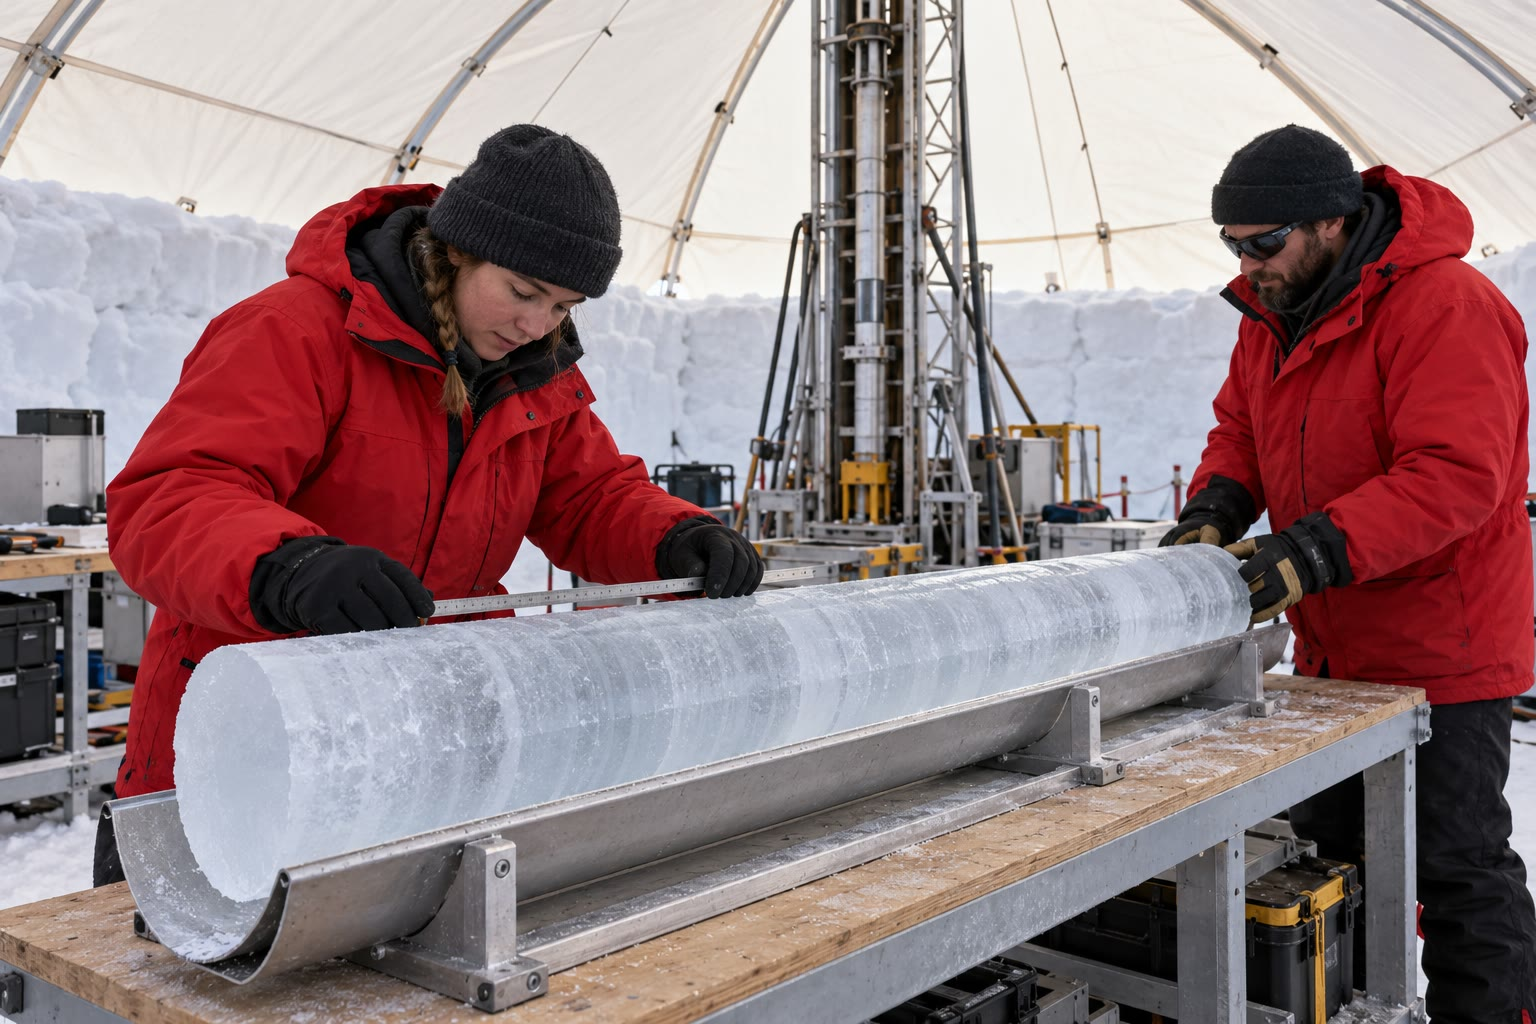
\includegraphics[width=\linewidth]{images/book5/ai/b3-ice-core-tent.jpg}

{\scriptsize Medición de un testigo de hielo en una cuna dentro de una tienda de perforación
sobre un casquete de hielo, con la torre de perforación al fondo (Ilustración generada por IA).}
\end{minipage}
\end{inthelab}

\section{Ejercicios}

\begin{exercise}[$\star$]\label{exo:b3:stable-isotopes:1}
Una calcita tiene $\delta^{18}\mathrm O = \qty{30.5}{\permil}$ y el agua en la que creció
\qty{-2.1}{\permil}, ambas referidas a VSMOW. Calcúlense $\alpha$, $1000\ln\alpha$ y
$\Delta$. ¿Cuánto difieren las dos últimas?
\end{exercise}

\begin{exercise}[$\star$]\label{exo:b3:stable-isotopes:2}
Una estación costera de alta latitud tiene una temperatura media anual de
\qty{-25}{\celsius}. Con las relaciones del capítulo para estaciones de este tipo,
prevéanse el $\delta^{18}\mathrm O$, el $\delta\mathrm D$ y el \omterm{def:b3:stable-isotopes:d-excess}{exceso de deuterio} de su
precipitación.
\end{exercise}
% ledger: dansgaard64:effects

\begin{exercise}[$\star$]\label{exo:b3:stable-isotopes:3}
En una cuenca, los carbonatos tienen $\delta^{13}\mathrm C = \qty{+1.0}{\permil}$ y la materia
orgánica, \qty{-26.0}{\permil}. Con aportes de \qty{-5}{\permil}, calcúlese
$f_{\mathrm{org}}$.
\end{exercise}
% ledger: planavsky22:forg

\begin{exercise}[$\star$]\label{exo:b3:stable-isotopes:4}
Una concha de braquiópodo tiene $\Delta_{47} = \qty{0.600}{\permil}$. Con la calibración
del capítulo, ¿a qué temperatura creció?
\end{exercise}
% ledger: isogeochem:d47

\begin{exercise}[$\star\star$]\label{exo:b3:stable-isotopes:5}
El vapor sale del océano con $\delta^{18}\mathrm O = \qty{-13}{\permil}$ y precipita
con un $\alpha = 1.0100$ constante. ¿Qué fracción de él queda cuando el
vapor alcanza \qty{-33}{\permil}? ¿Cuál es el $\delta^{18}\mathrm O$ de la lluvia
en ese momento?
\end{exercise}
% ledger: white13c9:rayleigh

\begin{exercise}[$\star\star$]\label{exo:b3:stable-isotopes:6}
La nieve de \qty{-40}{\permil} se compara con agua oceánica de 0. Calcúlense $\alpha$,
$1000\ln\alpha$, $1000(\alpha - 1)$ y $\Delta$ entre ambas. ¿Cuál de las
aproximaciones de la proposición no se cumple, y en cuánto?
\end{exercise}

\begin{exercise}[$\star\star$]\label{exo:b3:stable-isotopes:7}
Un foraminífero tiene $\delta^{18}\mathrm O = \qty{+1.50}{\permil}$ en VPDB y creció en
agua de \qty{0.00}{\permil} en VSMOW. Calcúlese su temperatura de crecimiento con el
método del capítulo y en cuánto modifica un error de \qty{0.1}{\permil} en el agua
la temperatura obtenida.
\end{exercise}
% ledger: isogeochem:ko97

\begin{exercise}[$\star\star$]\label{exo:b3:stable-isotopes:8}
El registro bentónico apilado cambia \qty{1.77}{\permil} desde el presente hasta el
Último Máximo Glacial. Elimínese la fracción de volumen de hielo calculada en el capítulo y
conviértase el resto en un cambio de temperatura de agua profunda, usando la pendiente de
la calibración de la calcita cerca de \qty{2}{\celsius}.
\end{exercise}
% ledger: data:lr04, white13c9:ice-volume, isogeochem:ko97

\begin{exercise}[$\star\star$]\label{exo:b3:stable-isotopes:9}
Una pirita tiene $\delta^{34}\mathrm S = \qty{10.0}{\permil}$ y $\delta^{33}\mathrm S =
\qty{8.2}{\permil}$. Calcúlese $\Delta^{33}\mathrm S$. ¿Qué indica sobre la
atmósfera cuando se formó la pirita?
\end{exercise}
% ledger: white13c9:s-mif

\begin{exercise}[$\star\star\star$]\label{exo:b3:stable-isotopes:10}
En la condensación en sistema cerrado, el vapor y todo el condensado formado permanecen
juntos en equilibrio. Demuéstrese que el vapor tiene entonces $R_v/R_{v,0} = 1/[f +
\alpha(1 - f)]$, y compárese con la \omterm{prop:b3:stable-isotopes:rayleigh-distillation}{destilación de Rayleigh} para $f = 0.2$ y
$\alpha = 1.01$.
\end{exercise}

\begin{exercise}[$\star\star\star$]\label{exo:b3:stable-isotopes:11}
A partir de la estimación de que \qty{2000}{Gt} de carbono de metano a
\qty{-60}{\permil} producen un desplazamiento de \qty{-2.5}{\permil} en el carbono intercambiable,
obténgase la masa del reservorio implícita, con $\delta_0 = 0$. Con esa masa, ¿cuánto
carbono orgánico a \qty{-25}{\permil} produce el mismo desplazamiento? Compárese con el
intervalo publicado.
\end{exercise}
% ledger: dickens11:petm

\begin{exercise}[$\star\star\star$]\label{exo:b3:stable-isotopes:12}
Demuéstrese que, a lo largo de una trayectoria de enfriamiento, $\mathrm d\delta_v/\mathrm dT = (\alpha - 1)(1000 +
\delta_v)\,\mathrm d\ln e_s/\mathrm dT$. A \qty{-20}{\celsius}, donde el
vapor del modelo del capítulo tiene $\delta^{18}\mathrm O = \qty{-49.1}{\permil}$
y la curva de sublimación da $\mathrm d\ln e_s/\mathrm dT =
\qty{0.0960}{K^{-1}}$. Calcúlese esta pendiente.
\end{exercise}
% ledger: gkinis14:alpha-ice, iapws:melt-subl

\section{Problema: el viaje de una gota de lluvia hasta Dome Ilse}

\begin{problem}[{Problema de fin de semana --- los isótopos de la nieve a lo largo de un
recorrido ficticio, una paleotemperatura y una excursión isotópica del carbono}]\label{pb:b3:stable-isotopes:1}
Una masa de aire sale del borde de un casquete de hielo ficticio a \qty{0}{\celsius}
con vapor de $\delta^{18}\mathrm O = \qty{-20.0}{\permil}$ y $\delta\mathrm D =
\qty{-150}{\permil}$, y se enfría a presión constante a medida que avanza hacia el interior.
La nieve se forma en la estación Coast a \qty{-10}{\celsius}, en Midway a
\qty{-20}{\celsius} y en Dome Ilse a \qty{-30}{\celsius}, cuando la fracción
de vapor que queda es $f = 0.425$, $0.169$ y $0.0622$. Úsense los factores de fraccionamiento
hielo--vapor del capítulo, constantes en cada tramo con el valor de
su temperatura media.
% ledger: gkinis14:alpha-ice, iapws:melt-subl, dansgaard64:effects, isogeochem:ko97, isogeochem:d47, white13c9:ice-volume, data:lr04, planavsky22:forg, dickens11:petm

\medskip\noindent\textbf{Parte I --- Destilación.}
\begin{enumerate}
\item Calcúlense $\alpha^{18}$ y $\alpha^{\mathrm D}$ a $-5$, $-10$, $-15$, $-20$,
$-25$ y \qty{-30}{\celsius} (cinco cifras significativas para el oxígeno, cuatro para
el deuterio).
\item Calcúlese el $\delta^{18}\mathrm O$ del vapor a su llegada a Coast.
\item Calcúlese el de la nieve de Coast.
\item Repítase para Midway (la razón de $f$ del tramo es $0.169/0.425$).
\item Repítase para Dome Ilse.
\item ¿Qué fracción del oxígeno-18 original del vapor sigue en el aire
en Dome Ilse?
\end{enumerate}

\medskip\noindent\textbf{Parte II --- Temperatura y deuterio.}
\begin{enumerate}[resume]
\item Calcúlese la pendiente del $\delta^{18}\mathrm O$ de la nieve frente a la
temperatura de condensación desde Coast hasta Dome Ilse.
\item ¿Qué temperatura superficial media anual asignaría la relación de las estaciones
de Groenlandia a la nieve de Dome Ilse? ¿Por qué puede diferir de
\qty{-30}{\celsius}?
\item Calcúlese el $\delta\mathrm D$ de la nieve en las tres estaciones del mismo modo.
\item Calcúlese su \omterm{def:b3:stable-isotopes:d-excess}{exceso de deuterio}. ¿Cómo cambia hacia el interior?
\item ¿Está la nieve de Dome Ilse sobre la recta de agua meteórica? ¿Qué omite
el modelo que sí incluye la formación real de nieve?
\end{enumerate}

\medskip\noindent\textbf{Parte III --- Un foraminífero frente a la costa.} Un
testigo de sedimento extraído frente a la costa proporciona foraminíferos bentónicos con \qty{3.25}{\permil}
VPDB en la parte superior y \qty{5.02}{\permil} en el Último Máximo Glacial; el agua de
fondo es hoy de \qty{0.00}{\permil} VSMOW.
\begin{enumerate}[resume]
\item Calcúlese la temperatura actual del agua de fondo con la calibración
de la calcita.
\item Calcúlese la temperatura glacial suponiendo que el agua no ha cambiado. ¿Es
posible el resultado?
\item Corríjase el agua glacial por un descenso del nivel del mar de \qty{125}{m} y
recalcúlese. ¿Cuál es el enfriamiento glacial del agua de fondo?
\item Calcúlese el $\Delta_{47}$ esperado a ambas temperaturas y su
diferencia.
\item ¿Por qué el termómetro de \omterm{def:b3:stable-isotopes:clumped}{isótopos agrupados} no necesita la composición del
agua?
\end{enumerate}

\medskip\noindent\textbf{Parte IV --- Una excursión de carbono.} Más abajo en el
testigo, los carbonatos de \qty{+0.5}{\permil} se interrumpen por una breve excursión de
\qty{-3.0}{\permil}.
\begin{enumerate}[resume]
\item Antes de la excursión, con $\delta_{\mathrm{in}} = \qty{-5}{\permil}$ y
$\Delta_B = \qty{-28}{\permil}$, calcúlese $f_{\mathrm{org}}$.
\item Tómese el depósito del ejercicio 11, \qty{46000}{Gt} en el instante 0. ¿Cuánto
carbono necesita la excursión si la fuente es metano a \qty{-60}{\permil}?
\item ¿Y si es carbono orgánico a \qty{-25}{\permil}?
\item ¿Y si es carbono del manto a \qty{-5}{\permil}?
\item ¿Qué observación en el mismo testigo podría ayudar a elegir entre
las fuentes?
\item Indíquese el $\delta^{18}\mathrm O$ de la nieve que cae en Dome Ilse.
\end{enumerate}
\end{problem}
